\section{课程介绍}

\begin{frame}
    \frametitle{课程所处地位}

    \begin{itemize}
        \item \textbf{《数据结构与算法》}是信息管理专业的\textcolor{red}{核心基础课程}之一。
        \item 它为学生提供解决实际问题和优化信息系统的\textcolor{red}{关键工具和技术}。
        \item 该课程与其他信息管理科学相关课程(如《管理信息系统》、《面向对象程序设计》、《商务智能与数据挖掘》、《信息系统分析与设计》等)相互关联,\textcolor{red}{构建了信息管理专业的技术基础}。
    \end{itemize}
    \begin{figure}
        \centering
        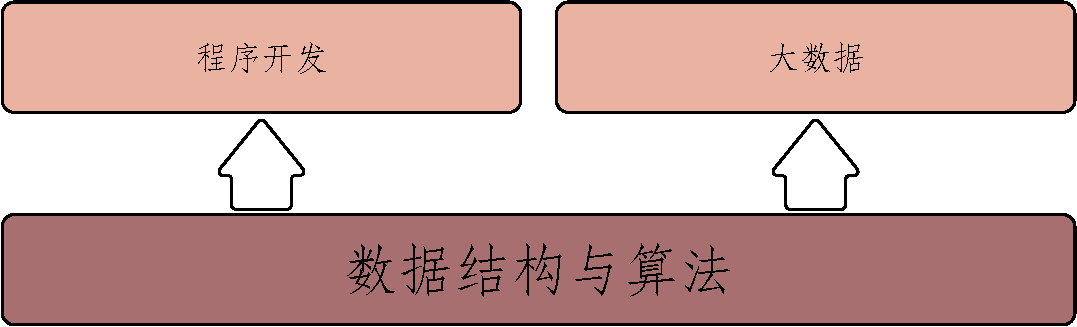
\includegraphics[width = 0.5\textwidth]{./images/import.pdf}
    \end{figure}

\end{frame}

\begin{frame}
    \frametitle{课程特征}

    \begin{itemize}
        \item \textbf{抽象性强}:数据结构与算法课程涉及到抽象的数据模型和算法设计,需要学生具备抽象思维和逻辑推理能力。
        \item \textbf{实践性强}:该课程注重实践操作和算法实现,学生需要通过编程实践来加深对数据结构和算法的理解和应用。
        \item \textbf{算法思维培养}:该课程强调培养学生的算法思维,即解决问题的思考方式和技巧,让学生具备分析、设计和优化算法的能力。
    \end{itemize}

\end{frame}

\begin{frame}
    \frametitle{主要讲授内容}

    \begin{itemize}
        \item 基本数据结构:包括数组、链表、栈、队列、树等常用数据结构的定义、实现和操作。
        \item 常用算法:涵盖排序算法、搜索算法、图算法等,如冒泡排序、快速排序、二分查找、广度优先搜索、最短路径算法等。
        \item 数据结构和算法的应用:介绍数据结构和算法在实际问题求解和信息管理系统中的应用,如数据库、大数据分析等领域。
    \end{itemize}

\end{frame}


\section{目标}

\begin{frame}
    \frametitle{期望目标}

    \begin{enumerate}
        \item 熟悉常见的数据集合抽象(例如栈、队列、列表、树、映射)。
        \item 理解实现常见数据结构的高效算法策略。
        \item 能够从理论和实验的角度分析算法性能,并识别不同策略之间的常见权衡和取舍。
        \item 能够基于Python语言明智地使用现有的数据结构和算法。
        \item 能够应用数据结构和算法解决复杂问题。
    \end{enumerate}

\end{frame}

\section{学习资源}

\begin{frame}
    \frametitle{学习资源}

    \begin{itemize}
        \item Cormen, T.H., Leiserson, C.E., Rivest, R.L., Stein, C., 2022. Introduction to Algorithms, 4th ed. The MIT Press.
        \item Goldwasser, M.H., Tamassia, R., Goodrich, M.T., 2018. Data Structures and Algorithms in Python. John Wiley \& Sons. \\ \vspace{\baselineskip}
        \item Guttag, J.V., 2021. Introduction to Computation and Programming Using Python, 3rd ed. The MIT Press. \\ \vspace{\baselineskip}
        \item Github: \href{https://github.com/TheAlgorithms}{The Algorithms - Python}
        \item VISUALGO: \href{https://visualgo.net/en}{visualgo}
    \end{itemize}

\end{frame}